\section{\textit{Web App}}

Neste capítulo é abordado o desenvolvimento da aplicação \textit{web}. É realizada uma introdução, apresentando os objetivos e funcionalidades da mesma. São mostrados detalhes relativos à utilização da aplicação e, de seguida, apresenta-se o modelo de arquitetura utilizado no desenvolvimento da mesma. Por fim, refere-se como aceder à aplicação e define-se o seu processo de \textit{deployment}.

\par \smallskip

A aplicação \textit{web} é responsável por estabelecer uma interface sobre a qual as organizações podem interagir com a plataforma, disponibilizando às mesmas ferramentas que possibilitam a realização de operações como por exemplo a criação de \textit{posts} ou a realização de pesquisas sobre a plataforma.

\par \smallskip

Foram definidos alguns requisitos chave no início da conceptualização da aplicação, como por exemplo:

\begin{itemize}
	\item disponibilizar meios para consultar os \textit{posts}, eventos e outros utilizadores da plataforma e interagir com os mesmos; 
	\item permitir às organizações editarem o seu perfil;
	\item possibilitar que as mesmas possam criar e editar \textit{posts} e eventos;
	\item apresentar contactos de voluntários interessados em eventos pertencentes à organização autenticada.
\end{itemize}

Numa fase inicial do projeto, foi considerada a opção de desenvolver a aplicação \textit{web} usando a \textit{framework} Angular.js. Contudo, após nova avaliação, optou-se por utilizar a tecnologia React. Esta alteração foi efetuada após verificar que React é a tecnologia mais usada no mercado à data da realização do projeto. 

\subsection{Utilização da web app}

Levando em consideração que este componente foi desenvolvido especificamente para organizações, a maioria das operações implicam que um utilizador organização esteja autenticado (através da interface demonstrada na Figura 9).

\begin{figure}[h]
	\centering
	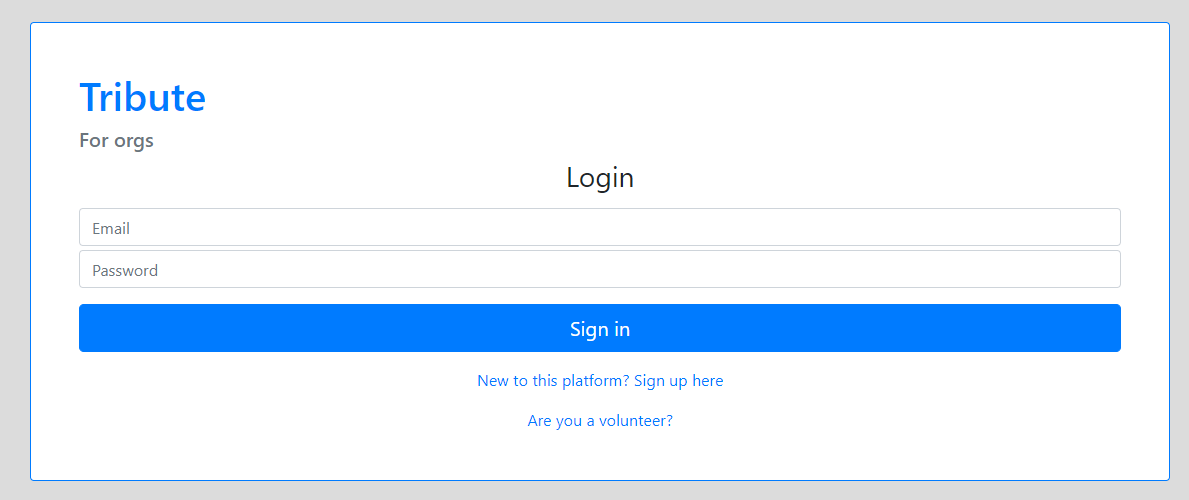
\includegraphics[scale=.31]{web_app_login_page}
	\caption{Interface de autenticação}
\end{figure}

Nesta versão da aplicação, é permitido que sejam registados utilizadores do tipo organização. Contudo, numa versão publicada da plataforma, o registo deste tipo de utilizadores seria realizado através do contacto direto dos mesmos com os gestores da aplicação de maneira a que apenas organizações fidedignas pudessem ter um perfil na plataforma.

\par \medskip

\begin{figure}[h]
	\centering
	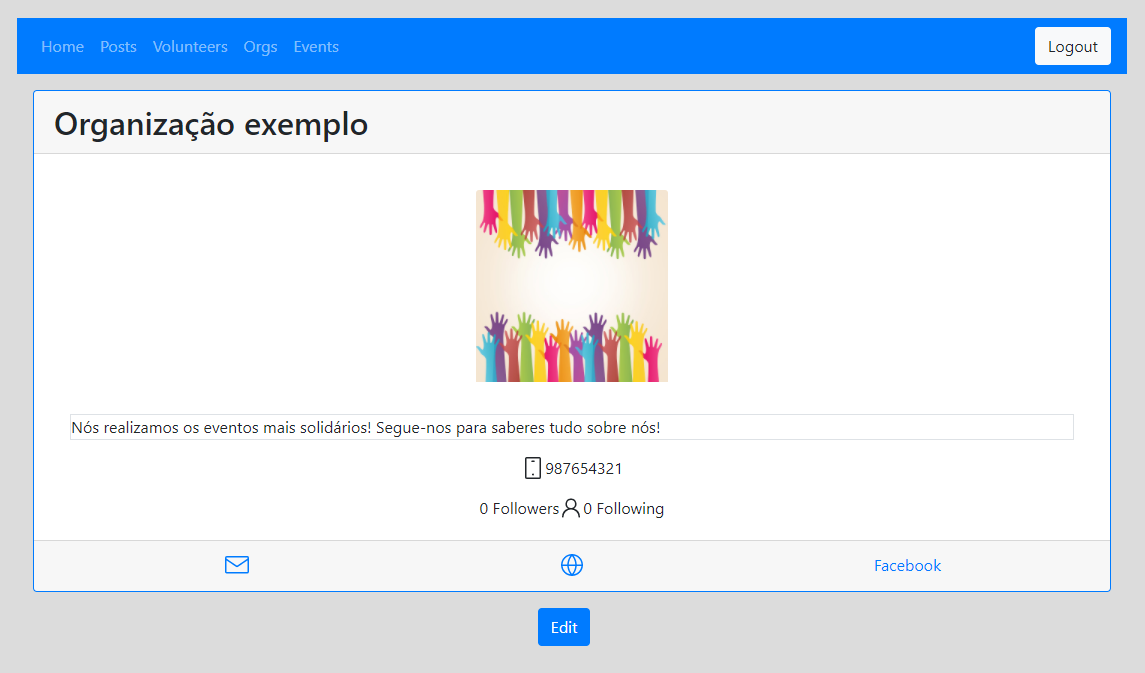
\includegraphics[scale=.31]{web_app_dashboard}
	\caption{Interface de autenticação}
\end{figure}

Após autenticação na aplicação, é disponibilizado um painel principal (consultar Figura 10) onde é possível navegar entre as várias páginas da aplicação e realizar as operações pretendidas.

\par \medskip

\subsection{Arquitetura}

A arquitetura da aplicação é composta principalmente por 2 módulos: API e Componentes e ainda a classe principal da aplicação.

\par \medskip 

Similar ao funcionamento do módulo com o mesmo nome na aplicação \textit{mobile}, API disponibiliza operações que realizam pedidos HTTPS à API. Componentes contém a implementação de todos os componentes \textit{react} apresentados ao utilizador, desde as páginas em si a componentes que são utilizados nestas. 

\par \medskip

A classe principal da aplicação é responsável não só por instanciar os serviços da API assim como definir o roteamento da aplicação \textit{web}.

\subsubsection{API}

A módulo API é composto por um conjunto de serviços que disponibilizam operações que necessitam de realizar pedidos HTTPS à API para serem realizadas (como por exemplo a solicitação de \textit{posts} ou a criação de um evento).

\par \medskip

Para cada entidade (voluntários, organizações, \textit{posts} e eventos) existe um serviço onde são definidas as operações possíveis de efetuar sobre a mesma. Todos os serviços utilizam uma classe auxiliar que contém a implementação de como efetuar pedidos HTTPS consoante o seu método (neste caso, GET, PUT, POST e DELETE). Esta classe auxiliar contém também a implementação de um requests

\subsubsection{Componentes}

Tal como já referido, o módulo Componentes é responsável por tratar a estruturação e apresentação da interface da aplicação assim como lidar com operações de \textit{input} por parte do utilizador. Como tal, este contém a definição de:

\begin{itemize}
	\item \textbf{componentes página}. Estes componentes definem os sub-componentes que constituem a página (por exemplo, na figura 11, a página dos eventos é constituída por um formulário para criar um novo evento e a lista dos eventos existentes na plataforma);
	\item \textbf{componentes específicos} por página, como por exemplo, uma lista de \textit{posts} ou um formulário para criar eventos;
	\item \textbf{componentes utilitários}, responsáveis por apresentar certos aspetos comuns da aplicação.
\end{itemize}

\begin{figure}[h]
	\centering
	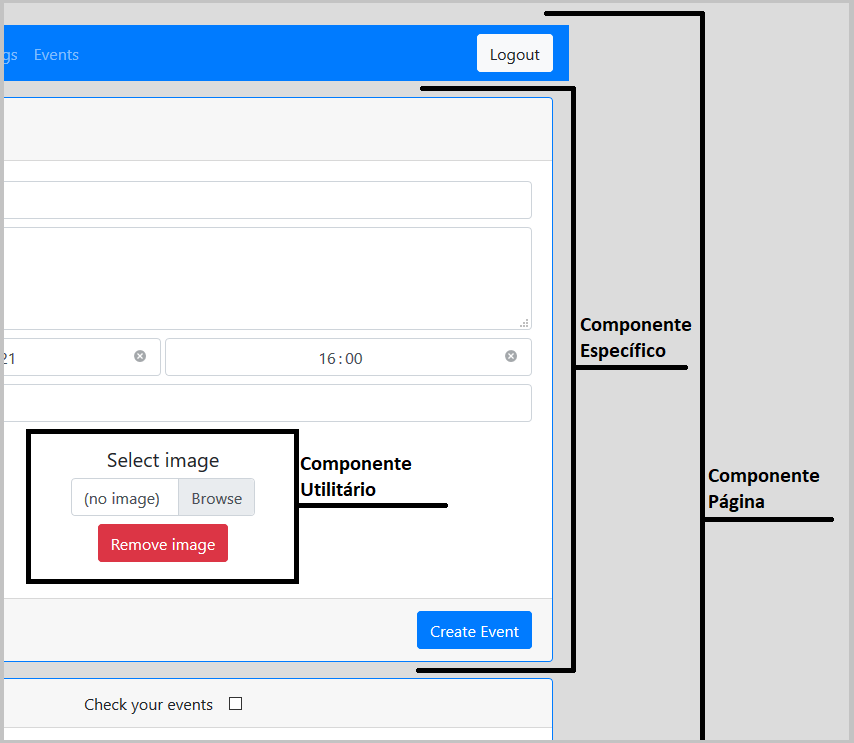
\includegraphics[scale=.38]{components_explained}
	\caption{Exemplo de tipos de componentes na página dos eventos}
\end{figure}

\bigskip

\subsubsection{Classe Principal}

A classe principal da aplicação instancia os serviços usados pelos componentes para efetuar pedidos à API e define também o roteamento da aplicação \textit{web}. No modo não autenticado, o acesso a quase todas as rotas da aplicação web é restringido. Apenas quando o cliente realiza autenticação com sucesso é permitido ao mesmo aceder às funcionalidades principais da aplicação.

\subsection{\textit{Deployment} da aplicação}

A aplicação foi \textit{deployed} utilizando uma máquina virtual do serviço \textit{Compute Engine} da \textit{Google Cloud Platform}. Foram instaladas as ferramentas necessárias para executar a aplicação nesta máquina (nomeadamente \textit{Node.js}) e a mesma encontra-se instanciada numa das portas da VM. 

\par \medskip

De maneira a lidar com pedidos CORS (Cross-Origin Resource Sharing), na máquina onde é executada a aplicação está instanciado um servidor \textit{web} Nginx. Este está configurado de maneira a redirecionar todos os pedidos que comecem com o preâmbulo /api para a máquina onde está \textit{deployed} a \textit{web} API. Todos os outros pedidos são redirecionados para a porta onde está a ser executada a aplicação \textit{web}.

\par \medskip

De maneira a associar um nome de domínio ao endereço IP da máquina onde está a ser executado o servidor \textit{web} foi utilizada a plataforma \textit{Duck DNS}, que permite reservar sem qualquer custo um número limitado de \textit{domain names}.

\par \medskip

Por fim, e utilizando as ferramentas disponibilizadas pela plataforma \textit{CertBot}, foi automaticamente emitido um certificado SSL e alterada a configuração do servidor \textit{Nginx} de maneira a que a plataforma aceitasse apenas comunicações através do protocolo HTTPS, garantindo segurança ponto-a-ponto entre máquina cliente e servidor \textit{web}.

\par \medskip

A aplicação encontra-se acessível em \url{https://tribute-app.duckdns.org/}.















































